%-----------------------------------------------------------------------------------------------%
%
% Maret 2019
% Template Latex untuk Tugas Akhir Program Studi Sistem informasi ini
% dikembangkan oleh Inggih Permana (inggihjava@gmail.com)
%
% Template ini dikembangkan dari template yang dibuat oleh Andreas Febrian (Fasilkom UI 2003).
%
% Orang yang cerdas adalah orang yang paling banyak mengingat kematian.
%
%-----------------------------------------------------------------------------------------------%

\chapter*{DAFTAR RIWAYAT HIDUP}
\pagestyle{empty}

\noindent

\begin{wrapfigure}{l}{3cm}
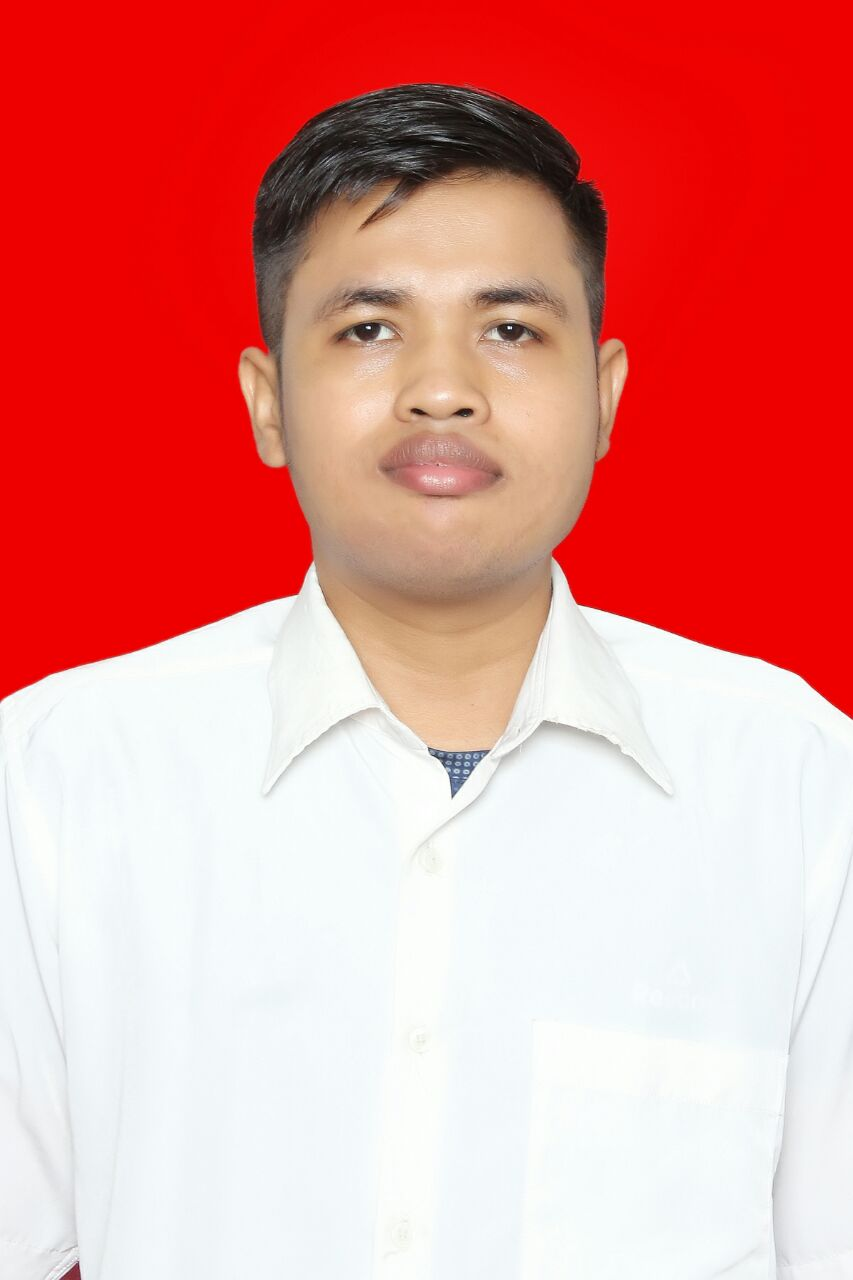
\includegraphics[width=3cm, height=4cm]{konten/gambar/fotoprofil.jpg}
\end{wrapfigure}


\penulisdua \ lahir pada tanggal 21 Januari 1995 Di Sebuah Kampung Kecil Bernama Ranah. Merupakan Anak ke 2 dari 3 bersaudara dari Pasangan Aguszaini dan Arnihar.
\inisial \ Memulai Pendidikan Dari Tingkat Dasar Pada SDN 020 Ranah (2001-2007) dan Melanjutkan pendidikan ke SLTP 1 Kampar (2007-2010), Lalu Melanjutkan Ke tingkat SLTA pada SMA N 1 Kampar(2010-2013). Saat ini \inisial \ sedang melanjutkan studi untuk mendapatkan gelar \gelar \ pada program studi \programStudi ,\ \fakultas ,\ \universitas \ (2013-2020).
jika tertarik ingin mengenal \inisial \ lebih lanjut, \inisial dapat ditemukan pada email \email \  atau silahkan hubungi pada jalur telepon di nomer \nohp